%-----------------------circuit 2--------------------------
\section{Single Phase Half Wave Controlled Rectifier with RLE load}

\subsection{Circuit used for simulation}

% figure that is centered on the page
\begin{figure}[h]
    \centering
    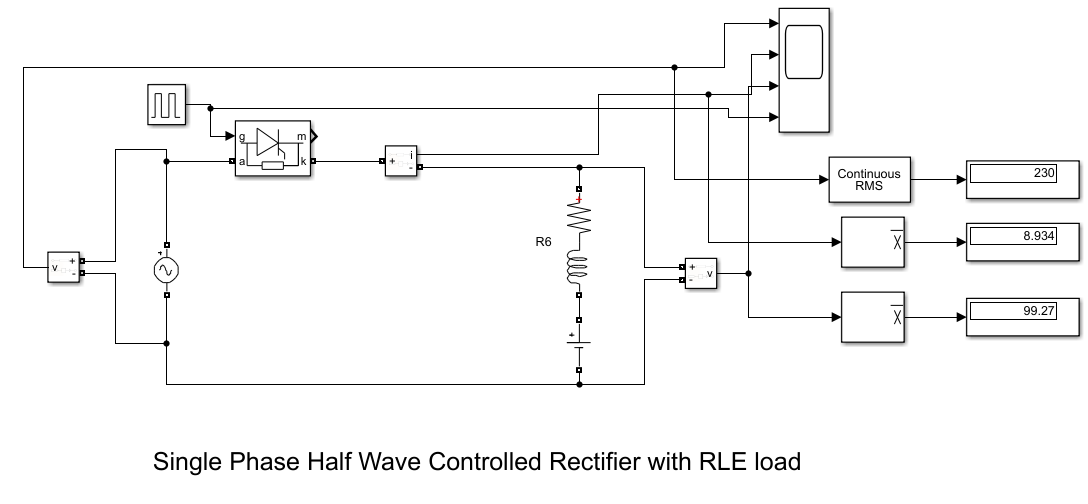
\includegraphics[width=0.7\textwidth]{images/experiment-1/circuit-diagram-simulation-07.png}
    \caption{Circuit used for simulation}
    \label{Fig_simulation_circuit_single-phase-half-wave-controlled-rectifier-with-RLE-load}
\end{figure}

\subsection{Components Required}

\begin{table}[h]
    \renewcommand{\arraystretch}{1.3}
    \label{table_components_required_circuit_7}
    \centering
    \begin{tabular}{|c|c|c|c|}
        \hline
        Sr. No & Parameters                     & Ratings            & Quantity \\
        \hline
        \hline
        1      & AC Single Phase Voltage Source & 230V ($ V_{rms} $) & 1        \\
        \hline
        2      & Resistor                       & 10$ \Omega $       & 1        \\
        \hline
        3      & Inductor                       & 10mH               & 1        \\
        \hline
        4      & Diode                          & -                  & 1        \\
        \hline
        5      & Voltmeter                      & -                  & 2        \\
        \hline
        6      & Ammeter                        & -                  & 1        \\
        \hline
        7      & Thyristor                      & -                  & 1        \\
        \hline
        8      & DC Source                      & 100V               & 1        \\
        \hline
    \end{tabular}
    \caption{Components for Single Phase Half Wave Controlled Rectifier with RLE load}

\end{table}

\pagebreak

\subsection{Observations}

\begin{table}[h]
    \renewcommand{\arraystretch}{1.3}
    \label{table_observation_7}
    \centering
    \begin{tabular}{|c|c|c|}
        \hline
        Parameters                              & Theoretical Values & Simulation Values \\
        \hline
        \hline
        AC Input Voltage ($ V_{in,rms} $)       & 230V               & 230V              \\
        \hline
        Output Average Voltage ($ V_{o,avg} $)  & 96.66V             & 155.1V            \\
        \hline
        Output Average Current ($ I_{o,avg}  $) & 9.66A              & 5.507A            \\
        \hline
        AC Input Power ($ P_{AC}  $)            & 2214.44 (W)        & 1266 (W)          \\
        \hline
        DC Input Power ($ P_{DC}  $)            & 926.98 (W)         & 853.9 (W)         \\
        \hline
        Efficiency (\%)                         & 41.86              & 67.43             \\
        \hline
    \end{tabular}
    \caption{Observations for Single Phase Half Wave Controlled Rectifier with RLE load}

\end{table}


After giving the firing gate pulse to the thyristor, the circuit begins to behave like an uncontrolled half wave rectifier with an RLE load. The output voltage waveform follows the same shape as the RLE load waveform, and the output current lags the output voltage due to the inductive component of the load.
The efficiency of controlled rectifier
with RL load is 67.43\%.



% \pagebreak


\subsection{Resultant Waveforms}

% figure that is centered on the page
\begin{figure}[h]
    \centering
    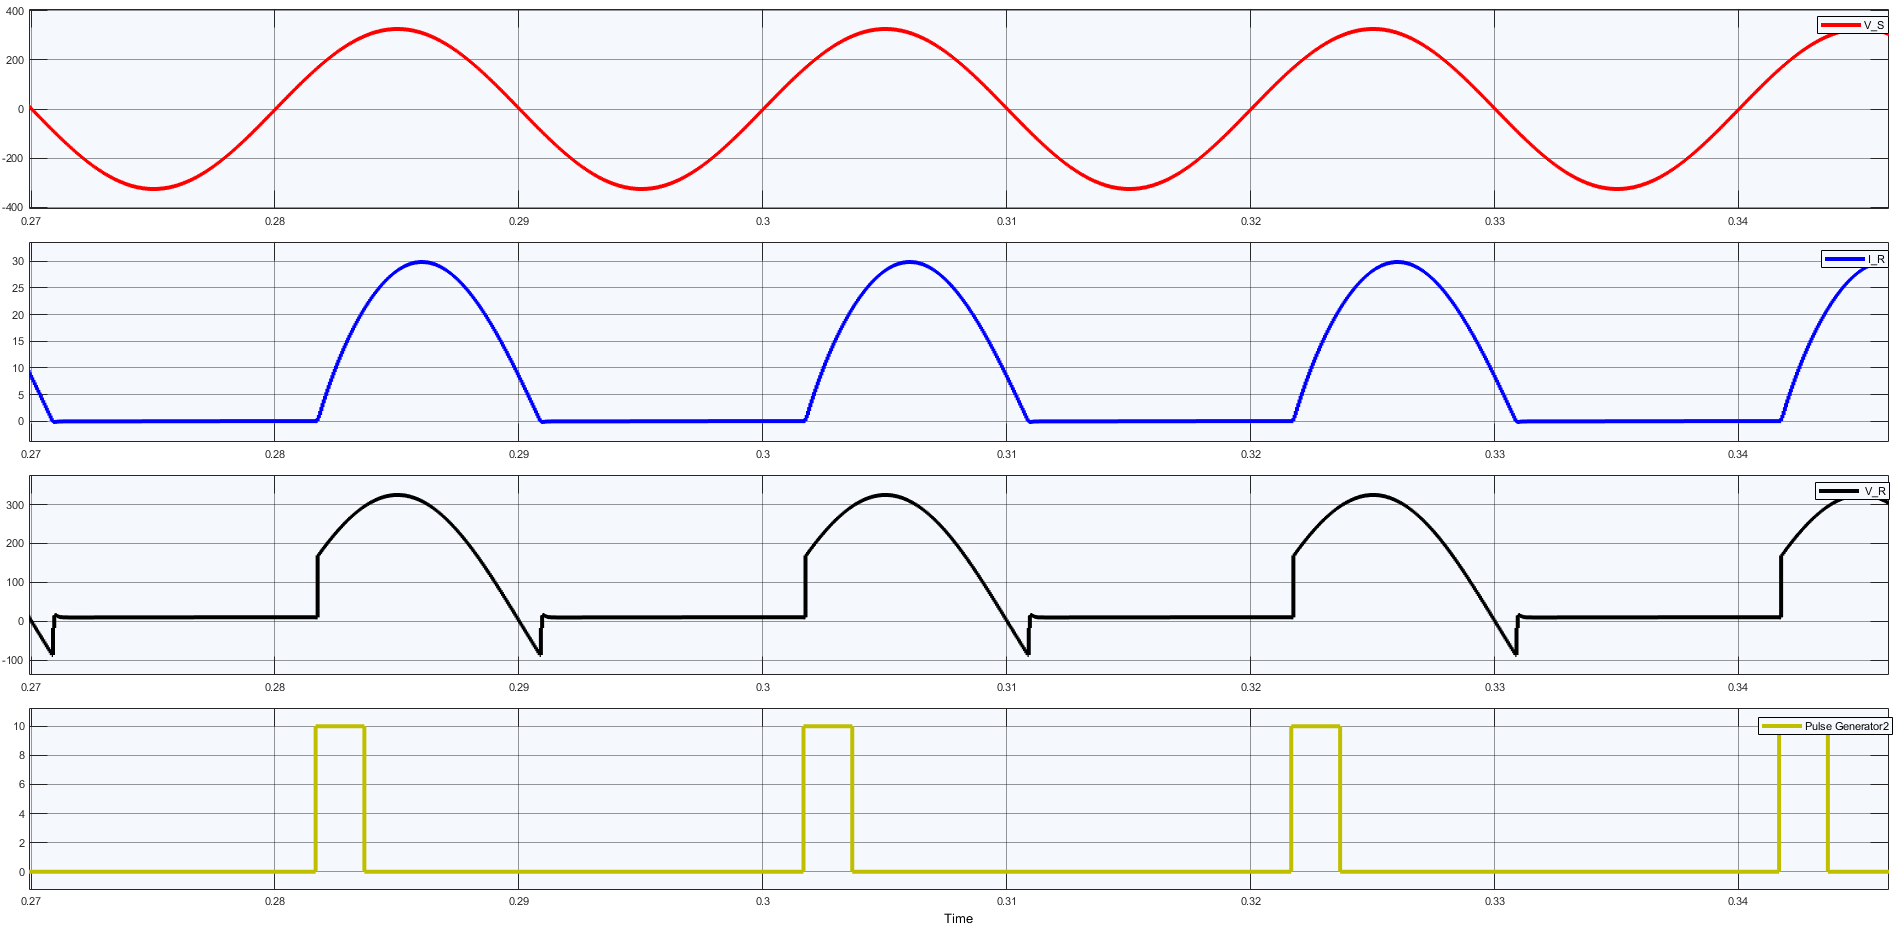
\includegraphics[width=1\textwidth]{images/experiment-1/circuit-scope-simulation-07.png}
    \caption{Scope Waveforms for Single Phase Half Wave Controlled Rectifier with RLE load}
    \label{Fig_waveform_single-phase-half-wave-controlled-rectifier-with-RLE-load}
\end{figure}


\pagebreak

